%!TEX root=../../main.tex
\begin{chapterpage}{The chi-square test}
  \chaptertitle{The chi-square test}
  \label{ch:chisquare}

  \chaptersection{twoWayTablesAndChiSquare}
  %\chaptersection{oneWayChiSquare}
  %\chaptersection{caseControStudies}
  %\chaptersection{infForPropNotes}
  \chaptersection{ChiExample}
  \chaptersection{ChiExercises}
\end{chapterpage}
\renewcommand{\chapterfolder}{ch_08a_inference_for_props_oi_biostat}

\chapterintro{{\large 
Two-way tables of two qualitative variables are often used to summarize data from medical research studies, and entire texts have been written about methods of analysis for these tables.  This chapter covers only the most basic of those methods.  }}


%__________________
\section{Inference for two or more groups}
\label{twoWayTablesAndChiSquare}

The comparison of the proportion of breast cancer deaths between the two groups can also be approached using a two-way contingency table, which contains counts for combinations of outcomes for two variables. The results for the mammogram study in this format are shown in Figure~\ref{mammogramStudySummaryTableWithTotals}. Each value in the table represents the number of times a particular combination of variable outcomes occurred. For example, the value 500 corresponds to the number of death from breast cancer (BC) in the group taking mammographs on a regular basis. Row and column totals are also included. The \term{row totals} \index{contingency table!row totals} provide the total counts across each row (e.g. $500+44,425 = 44,925$), and \term{column totals} \index{contingency table!column totals} are total counts down each column.



Previously, the main question of interest was stated as, "Is there evidence of a difference in the proportion of breast cancer deaths between the two screening groups?" If the probability of a death from breast cancer does not depend the method of screening, then screening method and outcome are independent. Thus, the question can be re-phrased: "Is there evidence that screening method is associated with outcome?"

Hypothesis testing in a two-way table assesses whether the two variables of interest are associated (i.e., not independent). The approach can be applied to settings with two or more groups and for responses that have two or more categories. The observed number of counts in each table cell are compared to the number of \term{expected counts}, where the expected counts are calculated under the assumption that the null hypothesis of no association is true. A $\chi^2$ test of significance is based on the differences between observed and expected values in the cells.

\begin{figure}[h]
	\centering
	\begin{tabular}{l| l l l l |l}
		\hline
		Death from BC & \hspace{1mm}  & Yes & No & \hspace{1mm} & Total \\
		\hline
		Mammogram				   &    & 500 & 44,425 & 				&44,925 \\
		Control				   &     & 505	& 44,405    &				& 44,910 \\
		\hline
		Total						   &    & 1,005 & 88,830 & 				& 89,835 \\
		\hline
	\end{tabular}
	\caption{Results of the mammogram study, as a contingency table with marginal totals.}
	\label{mammogramStudySummaryTableWithTotals}
\end{figure}

\begin{exercisewrap}
\begin{nexercise}
Formulate hypotheses for a contingency-table approach to analyzing the mammogram data.\footnotemark{}
\end{nexercise}
\end{exercisewrap}
\footnotetext{$H_0$: There is no association between type of breast cancer screening and death from breast cancer. $H_A$: There is an association between type of breast cancer screening and death from breast cancer.}


\subsection{Expected counts}
\label{twoWayTablesExpectedCounts}

If type of breast cancer screening had no effect on outcome in the mammogram data, what would the expected results be? 

Recall that if two events $A$ and $B$ are independent, then $P(A \cap B) = P(A)P(B)$. Let $A$ represent assignment to the mammogram group and $B$ the event of death from breast cancer. Under independence, the number of individuals out of 89,835 that are expected to be in the mammogram screening group and die from breast cancer equals:
\[(89,835) P(A)P(B) = (89,835) \left(\frac{44,925}{89,835}\right) \left(\frac{1,005}{89,835} \right) = 502.6. \]

Note that the quantities 44,925 and 1,005 are the row and column totals corresponding to the upper left cell of Figure~\ref{mammogramStudySummaryTableWithTotals}, and 89,835 is the total number $n$ of observations in the table. A general formula for computing expected counts for any cell can be written from the marginal totals and the total number of observations.

%\textD{\newpage}

\begin{onebox}{Computing expected counts in a two-way table}
To calculate the expected count for the $i^{th}$ row and $j^{th}$ column, compute
$$\text{Expected Count}_{\text{row }i,\text{ col }j} = \frac{(\text{row $i$ total}) \times  (\text{column $j$ total})}{\text{table total}}.\vspace{2mm}$$
\end{onebox}	
	
\begin{examplewrap}
\begin{nexample}{Calculate expected counts for the data in Figure~\ref{mammogramStudySummaryTableWithTotals}.}
\[E_{1,1} = \dfrac{44,925 \times 1,005}{89,835} = 502.6 \qquad E_{1,2} = \dfrac{44,925 \times 88,830}{89,835} = 44,422.4\]
\[E_{2,1} = \dfrac{2,922 \times 1,005}{89,835} = 502.4 \qquad E_{2,2} = \dfrac{7,078 \times 88,830}{89,835} = 44,407.6\]
\end{nexample}
\end{examplewrap}

\begin{figure}[h]
	\centering
		\begin{tabular}{l| l l l l| l}
			\hline
			Death from BC & \hspace{1mm}  & Yes & No & \hspace{1mm} & Total \\
			\hline
			Mammogram				   &    & 500 \highlightO{(502.6)} & 44,425  \highlightO{(44,422.4)} & 				&44,925 \\
			Control				   &     & 505  \highlightO{(502.4)}	& 44,405  \highlightO{(44,407.6)}  &				& 44,910 \\
			\hline
			Total						   &    & 1,005 & 88,830 & 				& 89,835 \\
			\hline
		\end{tabular}
	\caption{Results of the mammogram study, with \highlightO{(expected counts)}. The expected counts should also sum to the row and column totals; this can be a useful check for accuracy.}
	\label{mammogramStudyExpectedCounts}
\end{figure}

\index{data!hiv|(}

\begin{examplewrap}
\begin{nexample}{If a newborn is HIV$^+$, should he or she be treated with nevirapine (NVP) or a more expensive drug, lopinarvir (LPV)? In this setting, success means preventing virologic failure; i.e., growth of the virus. A randomized study was conducted to assess whether there is an association between treatment and outcome.\footnotemark{} Of the 147 children administered NVP, about 41\% experienced virologic failure; of the 140 children administered LPV, about 19\% experienced virologic failure. Construct a table of observed counts and a table of expected counts.}
	
Convert the proportions to count data: 41\% of 147 is approximately 60, and 19\% of 140 is approximately 27. The observed results are given in Figure~\ref{violariHivStudyObsCounts}.

Calculate the expected counts for each cell:
\[E_{1, 1} = \dfrac{87 \times 147}{287} = 44.6 \qquad E_{1, 2} = \dfrac{87 \times 140}{287} = 42.4 \]
\[E_{2, 1} = \dfrac{200 \times 147}{287} = 102.4 \qquad E_{2, 2} = \dfrac{200 \times 140}{287} = 97.6 \]

The expected counts are summarized in Figure~\ref{violariHivStudyExpCounts}.
\end{nexample}
\end{examplewrap}
\footnotetext{Violari A, et al. N Engl J Med 2012; 366:2380-2389
DOI: 10.1056/NEJMoa1113249}

\begin{figure}[h]
	\centering
	\begin{tabular}{l | l l | l}
	\hline
	& NVP & LPV & Total \\
	\hline
	Virologic Failure & 60 & 27 & 87 \\
	Stable Disease & 87 & 113 & 200 \\	
	\hline
	Total & 147 & 140 & 287 \\
	\hline
	\end{tabular}
	\caption{Observed counts for the HIV study.}
	\label{violariHivStudyObsCounts}
\end{figure}

\begin{figure}[h]
	\centering
	\begin{tabular}{l | l l | l}
		\hline
		& NVP & LPV & Total \\
		\hline
		Virologic Failure & 44.6 & 42.4 & 87 \\
		Stable Disease & 102.4 & 97.6 & 200 \\
		\hline	
		Total & 147 & 140 & 287 \\
		\hline
	\end{tabular}
	\caption{Expected counts for the HIV study.}
	\label{violariHivStudyExpCounts}
\end{figure}

\index{data!hiv|)}


%\textD{\newpage}


\subsection{The $\pmb{\chi^2}$ test statistic}

Previously, test statistics have been constructed by calculating the difference between a point estimate and a null value, then dividing by the standard error of the point estimate to standardize the difference. The $\chi^2$ statistic is based on a different idea.  In each cell of a table, the difference \emph{observed} - \emph{expected} is a measure of the discrepancy between what was observed in the data and what should have been observed under the null hypothesis of no association. If the row and column variables are highly associated, that difference will be large.  Two adjustments are made to the differences before the final statistic is calculated.  First, since both positive and negative differences suggest a lack of independence, the differences are squared to remove the effect of the sign.  Second, cells with larger counts may have larger discrepancies by chance alone, so the squared differences in each cell are scaled by the number expected in the cell under the hypothesis of independence.  The final $\chi^2$ statistic is the sum of these standardized squared differences, where the sum has one term for each cell in the table.

The $\chi^2$ test statistic\marginpar[\raggedright\vspace{9mm}

$\chi^2$\vspace{0.5mm}\\\footnotesize chi-square\\test statistic]{\raggedright\vspace{9mm}
	
	$\chi^2$\vspace{0.5mm}\\\footnotesize chi-square\\test statistic}\index{chi-square statistic} is calculated as:

\[\chi^2 = \sum_{\text{all cells}} \frac{(\text{observed} - \text{expected})^2}{\text{expected}}. \]

The theory behind the $\chi^2$ test and its sampling distribution relies on the same normal approximation to the binomial distribution that was introduced earlier.  The cases in the dataset must be independent and each expected cell count should be at least 10.  The second condition can be relaxed in tables with more than 4 cells.

\begin{onebox}{Conditions for the $\pmb{\chi^2}$ test}
Two conditions that must be checked before performing a $\chi^2$ test:
\begin{description}
\setlength{\itemsep}{0mm}
	\item[Independence.] Each case that contributes a count to the table must be independent of all the other cases in the table.
	\item[Sample size.] Each expected cell count must be greater than or equal to 10. For tables larger than $2 \times 2$, it is appropriate to use the test if no more than 1/5 of the expected counts are less than 5, and all expected counts are greater than 1.
\end{description}
\end{onebox}


\begin{examplewrap}
\begin{nexample}{For the mammogram data, check the conditions for the $\chi^2$ test and calculate the $\chi^2$ test statistic.}

Independence is a reasonable assumption, since individuals have been randomized to either the treatment or control group. Each expected cell count is greater than 10.
\begin{align*}
\chi^2 &= \sum_{\text{all cells}} \frac{(\text{observed} - \text{expected})^2}{\text{expected}} \\
&= \dfrac{(500 - 502.6)^2}{502.6} + \dfrac{(44,425 - 44,422.4)^2}{44,422.4} + \dfrac{(505 - 502.4)^2}{502.4} + \dfrac{(44,405 - 44,407.6)^2}{44,407.6} \\
&=0.02.
\end{align*}	
\end{nexample}
\end{examplewrap}

\begin{exercisewrap}
\begin{nexercise}
For the HIV data, check the conditions for the $\chi^2$ test and calculate the $\chi^2$ test statistic.\footnotemark{}
\end{nexercise}
\end{exercisewrap}
\footnotetext{Independence holds, since this is a randomized study. The expected counts are greater than 10. $\chi^2 = \frac{(60-44.6)^2}{44.6} + \frac{(27-42.4)^2}{42.4} + \frac{(87-102.4)^2}{102.4} + \frac{(113-97.6)^2}{97.6} = 14.7.$}


\subsection{Calculating $\pmb{\MakeLowercase{p}}$-values for a $\pmb{\chi^2}$ distribution}

The \term{chi-square distribution} is often used with data and statistics that are positive and right-skewed.  The distribution is characterized by a single parameter, the degrees of freedom. Figure~\ref{chiSquareDistributionWithInceasingDF} demonstrates three general properties of chi-square distributions as the degrees of freedom increases: the distribution becomes more symmetric, the center moves to the right, and the variability increases.

\begin{figure}[h]
	\centering
	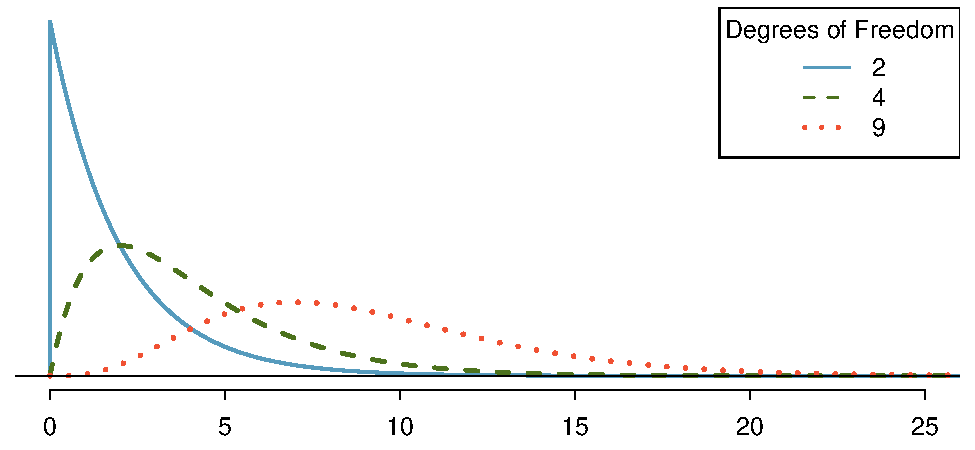
\includegraphics[width=0.9\textwidth]{ch_08a_inference_for_props_oi_biostat/figures/chiSquareDistributionWithInceasingDF/chiSquareDistributionWithInceasingDF}
	\caption{Three chi-square distributions with varying degrees of freedom.}
	\label{chiSquareDistributionWithInceasingDF}
\end{figure}

%\textD{\newpage}

The $\chi^2$ statistic from a contingency table has a sampling distribution that approximately follows a $\chi^2$ distribution with degrees of freedom $df = (r-1)(c-1)$, where $r$ is the number of rows and $c$ is the number of columns. Either statistical software or a table can be used to calculate $p$-values from the $\chi^2$ distribution. The \term{chi-square table} is partially shown in Figure~\ref{chiSquareProbabilityTableShort}, and a more complete table is presented in Appendix~\vref{chiSquareProbabilityTable}. This table is very similar to the $t$-table: each row provides values for distributions with different degrees of freedom, and a cut-off value is provided for specified tail areas. One important difference from the $t$-table is that the $\chi^2$ table only provides upper tail values.

\begin{figure}[h]
	\centering
	\begin{tabular}{r | rrrr | rrrr |}
		\hline
		Upper tail & 0.3 & 0.2 & 0.1 & 0.05 & 0.02 & 0.01 & 0.005 & 0.001 \\ 
		\hline
		df \hfill 1 & \footnotesize 1.07 & \footnotesize 1.64 & \footnotesize 2.71 & \footnotesize 3.84 & \footnotesize 5.41 & \footnotesize 6.63 & \footnotesize 7.88 & \footnotesize 10.83 \\ 
		\hfill 2 & \footnotesize 2.41 & \footnotesize 3.22 & \footnotesize 4.61 & \footnotesize 5.99 & \footnotesize 7.82 & \footnotesize 9.21 & \footnotesize 10.60 & \footnotesize 13.82 \\ 
		3 & \footnotesize 3.66 & \footnotesize 4.64 & \footnotesize 6.25 & \footnotesize 7.81 & \footnotesize 9.84 & \footnotesize 11.34 & \footnotesize 12.84 & \footnotesize 16.27 \\ 
		4 & \footnotesize 4.88 & \footnotesize 5.99 & \footnotesize 7.78 & \footnotesize 9.49 & \footnotesize 11.67 & \footnotesize 13.28 & \footnotesize 14.86 & \footnotesize 18.47 \\ 
		5 & \footnotesize 6.06 & \footnotesize 7.29 & \footnotesize 9.24 & \footnotesize 11.07 & \footnotesize 13.39 & \footnotesize 15.09 & \footnotesize 16.75 & \footnotesize 20.52 \\ 
		\hline
		6 & \footnotesize 7.23 & \footnotesize 8.56 & \footnotesize 10.64 & \footnotesize 12.59 & \footnotesize 15.03 & \footnotesize 16.81 & \footnotesize 18.55 & \footnotesize 22.46 \\ 
		7 & \footnotesize 8.38 & \footnotesize 9.80 & \footnotesize 12.02 & \footnotesize 14.07 & \footnotesize 16.62 & \footnotesize 18.48 & \footnotesize 20.28 & \footnotesize 24.32 \\ 
		\hline
	\end{tabular}
	\caption{A section of the chi-square table. A complete table is in Appendix~\vref{chiSquareProbabilityTable}.}
	\label{chiSquareProbabilityTableShort}
\end{figure}

\begin{examplewrap}
\begin{nexample}{Calculate an approximate $p$-value for the mammogram data, given that the $\chi^2$ statistic equals 0.02. Assess whether the data provides convincing evidence of an association between screening group and breast cancer death.}

The degrees of freedom in a $2 \times 2$ table is 1, so refer to the values in the first column of the probability table. The value 0.02 is less than 1.07, so the $p$-value is greater than 0.3. The data do not provide convincing evidence of an association between screening group and breast cancer death. This supports the conclusions from Example~\ref{mammogramExProp}, where the $p$-value was calculated to be 0.8650 and is visualized in Figure~\ref{mammogramPValue}.
\end{nexample}
\end{examplewrap}

\begin{figure}[h]
	\centering
	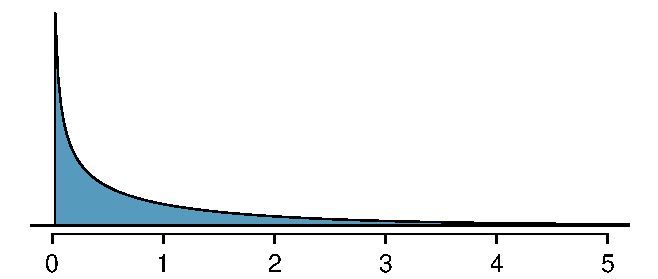
\includegraphics[width=0.6\textwidth]{ch_08a_inference_for_props_oi_biostat/figures/mammogramPValue/mammogramPValue}
	\caption{The $p$-value for the mammogram data is shaded on the $\chi^2$ distribution with $df=1$.The shaded area is to the right of x = 0.02.}
	\label{mammogramPValue}
\end{figure}

\begin{exercisewrap}
\begin{nexercise}\label{hivDataPValue}%
Calculate an approximate $p$-value for the HIV data. Assess whether the data provides convincing evidence of an association between treatment and outcome at the $\alpha = 0.01$ significance level.\footnotemark{}
\end{nexercise}
\end{exercisewrap}
\footnotetext{The $\chi^2$ statistic is 14.7. For degrees of freedom 1, the tail area beyond 14.7 is smaller than 0.001. There is evidence to suggest that treatment is not independent of outcome.}


%\textD{\newpage}


\subsection{Interpreting the results of a $\pmb{\chi^2}$ test}

If the $p$-value from a $\chi^2$ test is small enough to provide evidence to reject the null hypothesis of no association, it is important to explore the results further to understand direction of the observed association. This is done by examining the residuals, the standardized differences of the \emph{observed} - \emph{expected}, for each cell. Instead of using squared differences, the residuals are based on the differences themselves, and the standardizing or scaling factor is $\sqrt{\text{expected}}$.  Calculating residuals can be particularly helpful for understanding the results from large tables.

\index{residuals!contingency table}

For each cell in a table, the residual equals:
\[\dfrac{\text{observed} - \text{expected}}{\sqrt{\text{expected}}}. \]
Residuals with a large magnitude contribute the most to the $\chi^2$ statistic. If a residual is positive, the observed value is greater than the expected value, and vice versa for a negative residual.

\index{data!famuss|(}

\section{Examples of the chi-square test}
\label{ChiExample}
\begin{examplewrap}
  \begin{nexample}
    {In the FAMuSS study introduced in Chapter~\ref{introductionToData}, researchers measured a variety of demographic and genetic characteristics for about 1,300 participants, including data on race and genotype at a specific locus on the ACTN3 gene (Figure~\ref{famussObservedCountsRaceGenotype}).
    Is there evidence of an association between genotype and race?} First, check the assumptions for applying a $\chi^2$ test. It is reasonable to assume independence, since it is unlikely that any participants were related to each other. None of the expected counts, as shown in Figure~\ref{famussExpectedRaceGenotype}, are less than 5.

$H_0$: Race and genotype are independent.

$H_A$: Race and genotype are not independent.

Let $\alpha = 0.05$.

Calculate the $\chi^2$ statistic:
\begin{align*}
\chi^2 &= \sum_{\text{all cells}} \frac{(\text{observed} - \text{expected})^2}{\text{expected}} \\
&= \dfrac{(16-7.85)^2}{7.85} + \dfrac{(6-11.84)^2}{11.84} + ... + \dfrac{(5 - 6.22)^2}{6.22} \\
&=19.4.
\end{align*}	

Calculate the $p$-value: for a table with 3 rows and 5 columns, the $\chi^2$ statistic is distributed with $(3-1)(5-1) = 8$ degrees of freedom. From the table, a $\chi^2$ value of 19.4 corresponds to a tail area between 0.01 and 0.02. Thus, there is sufficient evidence to reject the null hypothesis of independence between race and genotype.

The $p$-value can be obtained using the \textsf{R} function \texttt{pchisq} (\texttt{pchisq(19.4, df = 8, lower.tail = FALSE)}), which returns a value of 0.012861. %\footnote{\texttt{pchisq(19.4, df = 8, lower.tail = FALSE)}}

To further explore the differences in genotype distribution between races, calculate residuals for each cell (Figure~\ref{famussResidualsRaceGenotype}). The largest residuals are in the first row; there are many more African Americans with the CC genotype than expected under independence, and fewer with the CT genotype than expected. The residuals in the second row indicate a similar trend for Asians, but with a less pronounced difference. These results suggest further directions for research; a future study could enroll a larger number of African American and Asian participants to examine whether the observed trend holds with a more representative sample. Geneticists might also be interested in exploring whether this genetic difference between populations has an observable phenotypic \mbox{effect}.
\end{nexample}
\end{examplewrap}

% latex table generated in R 3.2.4 by xtable 1.8-2 package
% Wed Dec 07 22:13:57 2016
\begin{figure}[ht]
	\centering
	\begin{tabular}{r | l l l | l}
		\hline
		& CC & CT & TT & Sum \\ 
		\hline
		African American & 16 & 6 & 5 & 27 \\ 
		Asian & 21 & 18 & 16 & 55 \\ 
		Caucasian & 125 & 216 & 126 & 467 \\ 
		Hispanic & 4 & 10 & 9 & 23 \\ 
		Other & 7 & 11 & 5 & 23 \\ 
		\hline
		Sum & 173 & 261 & 161 & 595 \\ 
		\hline
	\end{tabular}
	\caption{Observed counts for race and genotype data from the FAMuSS study.}
    \label{famussObservedCountsRaceGenotype}
\end{figure}
%labels modified from xtable

% latex table generated in R 3.2.4 by xtable 1.8-2 package
% Thu Dec 08 10:34:51 2016
\begin{figure}[ht]
	\centering
	\begin{tabular}{r| l l l | l}
		\hline
		& CC & CT & TT & Sum \\ 
		\hline
		African Am & 7.85 & 11.84 & 7.31 & 27.00 \\ 
		Asian & 15.99 & 24.13 & 14.88 & 55.00 \\ 
		Caucasian & 135.78 & 204.85 & 126.36 & 467.00 \\ 
		Hispanic & 6.69 & 10.09 & 6.22 & 23.00 \\ 
		Other & 6.69 & 10.09 & 6.22 & 23.00 \\ 
		\hline
		Sum & 173.00 & 261.00 & 161.00 & 595.00 \\ 
		\hline
	\end{tabular}
	\caption{Expected counts for race and genotype data from the FAMuSS study.}
	\label{famussExpectedRaceGenotype}
\end{figure}
%labels and formatting modified

% latex table generated in R 3.2.4 by xtable 1.8-2 package
% Thu Dec 08 10:48:57 2016
\begin{figure}[ht]
	\centering
	\begin{tabular}{r|lll|l}
		\hline
		& CC & CT & TT & Sum \\ 
		\hline
		African Am & \highlightO{2.91} & \highlightO{-1.70} & -0.85 & 0.00 \\ 
		Asian & \highlightO{1.25} & \highlightO{-1.25} & 0.29 & 0.00 \\ 
		Caucasian & -0.93 & 0.78 & -0.03 & 0.00 \\ 
		Hispanic & -1.04 & -0.03 & 1.11 & 0.00 \\ 
		Other & 0.12 & 0.29 & -0.49 & 0.00 \\ 
		\hline
		Sum & 0.00 & 0.00 & 0.00 & 0.00 \\ 
		\hline
	\end{tabular}
	\caption{Residuals for race and genotype data from the FAMuSS study.}
     \label{famussResidualsRaceGenotype}
\end{figure}

\index{data!famuss|)}
\index{data!hiv}

\begin{examplewrap}
\begin{nexample}{In Guided Practice~\ref{hivDataPValue}, the $p$-value was found to be smaller than 0.001, suggesting that treatment is not independent of outcome. Does the evidence suggest that infants should be given nevirapine or lopinarvir?}\label{HIVDirectionEx}%

In a $2 \times 2$ table, it is relatively easy to directly compare observed and expected counts. 
For nevirapine, more infants than expected experienced virologic failure (60 > 44.6), while fewer than expected reached a stable disease state (87 < 102.4). For lopinarvir, fewer infants than expected experienced virologic failure (27 < 42.4), and more infants than expected reached a stable disease state (113 > 97.6) (Figure~\ref{observedAndExpectedCountsForTheHivStudy}). The outcomes for infants on lopinarvir are better than for those on nevirapine; combined with the results of the significance test, the data suggest that lopinarvir is associated with better treatment outcomes.
\end{nexample}
\end{examplewrap}

\begin{figure}[h]
	\centering
	\begin{tabular}{l | l l | l}
		\hline
		& NVP & LPV & Total \\
		\hline
		Virologic Failure & 60 \highlightO{44.6} & 27 \highlightO{42.4} & 87 \\
		Stable Disease & 87 \highlightO{102.4} & 113 \highlightO{97.6}& 200 \\	
		\hline
		Total & 147 & 140 & 287 \\
		\hline
	\end{tabular}
	\caption{Observed and \highlightO{(expected)} counts for the HIV study.}
	\label{observedAndExpectedCountsForTheHivStudy}
\end{figure}			
		
\begin{exercisewrap}
\begin{nexercise}
Confirm the conclusions reached in Example~\ref{HIVDirectionEx} by analyzing the residuals.\footnotemark{}
\end{nexercise}
\end{exercisewrap}
\footnotetext{$R_{1, 1} = \frac{(44.6-60)}{\sqrt{44.6}} = 2.31$; $R_{1, 2} = \frac{(42.4-27)}{\sqrt{27}} = -2.37$; $R_{2, 1} = \frac{(87-102.4)}{\sqrt{102.4}} = -1.53$; $R_{2, 2} = \frac{(113-97.6)}{\sqrt{97.6}} = 1.56$. The positive residuals for the upper left and lower right cells indicate that more infants than expected experienced virologic failure on NVP and stable disease on LPV; vice versa for the upper right and lower left cells. The larger magnitude of the residuals for the two NVP cells indicates that most of the discrepancy between observed and expected counts is for outcomes related to NVP.}

\index{data!LEAP}

\begin{exercisewrap}
\begin{nexercise}
Chapter~\ref{introductionToData} started with the discussion of a study examining whether exposure to peanut products reduce the rate of a child developing peanut allergies. Children were randomized either to the peanut avoidance or the peanut consumption group; at 5 years of age, each child was tested for peanut allergy using an oral food challenge (OFC). The results of the OFC are reproduced in Figure~\ref{leapStudyResultsTest}; failing the food challenge indicates an allergic reaction. Assess whether there is evidence for exposure to peanut allergy reducing the chance of developing peanut allergies.\footnotemark{}
\end{nexercise}
\end{exercisewrap}
\footnotetext{The assumptions for conducting a $\chi^2$ test are satisfied. Calculate a $\chi^2$ test statistic: 24.29. The associated $p$-value is $8.3 \times 10^{-7}$. There is evidence to suggest that treatment group is not independent of outcome. Specifically, a residual analysis shows that in the peanut avoidance group, more children than expected failed the OFC; in the peanut consumption group, more children than expected passed the OFC.}

  
\textD{\newpage}

\begin{examplewrap}
  \begin{nexample}{
    
The objective of a study is to identify factors of
  postpartum endometritis in dairy cows. One of the factors of the
  study is the breed of the cow. The study has been performed between
  Holstein--Friesian, Jersey and the crossbreed between them. Two
  variables were considered: breed (3 possible values:
  Holstein--Friesian, Jersey and crossbreed) and whether they suffer
  from endometritis. 

For the study a sample of  300 dairy cattles have been selected. The result of the
analysis have been the following
11 out of 50
Holstein--Friesian have endometritis, 
7 out of 50 Jersey cows and 12 out of 200 crossbreed cows suffer from
this symptom.  These data are summarized in the contingency table of Figure~\ref{tab:cowsEndo}
}


What the study is trying to assess is whether there exists a statistically significant evidence that the breed of the cattle is going to be an independent factor of endometritis or there exists a relation between the two variables.  It's important to say that a relation between the two variables does not mean that one variable is the cause of the other variable. It's possible to find multiple relation between variable and none of this variable is the cause of the other. Therefore, the null and alternative hypothesis are the following: 

  $$\left \{ 
    \begin{array}{ll}
      H_0: &  \text{Breed and endometritis are independent (non--association)} \\
      H_1: & \text{Breed and endometritis are dependent (association)}
    \end{array} \right .
$$ 


In Table~\ref{tab:ColPropCow} is shown a column proportion table and it can be seen that the proportion of endometritis between the three groups are quite different. So, it can be thougth that breeds and endometritis are dependent variables, but a more accurate method is using the chi--square statistic.  



The expected value for every cell  is calculated
and a contingency table with this information is on the table below

\begin{align*} 
      E_{\text{Non-End},\text{HF}}& =
      \frac{O_{\text{Non-End},\bullet}\cdot
                                    O_{\bullet,\text{HF}}}{n}=\frac{270\cdot 50}{300}=45.00 &  E_{\text{End},\text{HF}}& =
      \frac{O_{\text{End},\bullet}\cdot  O_{\bullet,\text{HF}}}{n}=30\cdot \frac{50}{ 300}=5.00 \\
  E_{\text{Non-End},\text{J}}& =
  \frac{O_{\text{Non-End},\bullet} \cdot O_{\bullet,\text{J}}}{n}
=\frac{270\cdot 50}{300}=45.00  &   E_{\text{End},\text{J}}& =
  \frac{O_{\text{End},\bullet} \cdot O_{\bullet,\text{J}}}{n}
=\frac{30\cdot 50}{300}=5.00 \\
  E_{\text{Non-End},\text{CB}}& =
  \frac{E_{\text{Non-End},\bullet}\cdot
                                E_{\bullet,\text{CB}}}{n}=\frac{270\cdot 200}{300}=180.00 &
   E_{\text{End},\text{HF}}& =
  \frac{E_{\text{End},\bullet}\cdot
                            E_{\bullet,\text{HF}}}{n}=\frac{30\cdot 200 }{300}=20.00 
    \end{align*}
  \begin{tabular}{l|lll|l}
   \hline  & Holstein--Friesian & Jersey & Crossbreed & Total \\ 
 \hline No endometritis &  45 & 45 & 180 & 270 \\
Endometritis & 5 & 5 & 20 & 30 \\
\hline Total & 50 & 50 & 200 & \\
\hline 
  \end{tabular}


The $\chi^2$ test statistic of the contingency table of the variables
endometritis and breeds of the cows is calculated 
\begin{align*}
  x^2
  =&\frac{(39-45)^2}{45}+\frac{(43-45)^2}{45}+\frac{(188-180)^2}{180}+
  \frac{(11-5)^2}{5}+\frac{(7-7)^2}{7}+\frac{(12-20)^2}{20}=\\
=&
  \frac{36}{45}+\frac{4}{45}+\frac{64}{180}+\frac{36}{5}+\frac{4}{5}+\frac{64}{20}=\frac{2240}{180}=12.4444
\end{align*}


The degree of freedom is $df=(R-1)\cdot (C-1)=1\cdot 2 = 2$ and the critical value is $\chi_{2,.95}=5.99$. 
Hence, the acceptance interval is $(0,5.99)$. 
The value 12.44 is outside of
the interval. Therefore, the null hypothesis is rejected. It means that there exists enough evidence that breeds and postpartum endometritis are dependent variables and the proportions of endometritis is not the same between the breeds.   
\end{nexample}
\end{examplewrap}
 % latex table generated in R 3.1.1 by xtable 1.7-4 package
% Thu Jul 16 07:12:04 2015
\begin{figure}[h]
	\centering
	\begin{tabular}{rrrr}
		\hline
		& FAIL OFC & PASS OFC & Sum \\ 
		\hline
		Peanut Avoidance & 36 & 227 & 263 \\ 
		Peanut Consumption & 5 & 262 & 267 \\ 
		Sum & 41 & 489 & 530 \\ 
		\hline
	\end{tabular}
	\caption{LEAP Study Results.} 
	\label{leapStudyResultsTest}
\end{figure}
%library(xtable); outcome.table = addmargins(table(LEAP$treatment.group, LEAP$overall.V60.outcome)); xtable(outcome.table, digits = 0, caption = "LEAP Study Results", caption  = "leapStudyResults")


\begin{figure}[h]
  \begin{center}
    \begin{tabular}{l|lll|l}
   \hline  & Holstein--Friesian & Jersey & Crossbreed & Total \\ 
 \hline No endometritis &  39 & 43 & 188 & 270 \\
\cline{1-1} Endometritis & 11 & 7 & 12 & 30 \\
\hline Total & 50 & 50 & 200 & \\
\hline 
  \end{tabular}
    \end{center}
  \caption{Contingency table of the cows suffering from endometritis depending on the breed.}
\label{tab:cowsEndo}
\end{figure}


\begin{figure}[h]

   \begin{tabular}{l|lll|l}
   \hline  & Holstein--Friesian & Jersey & Crossbreed & Total \\ 
 \hline No endometritis &  0.78 & 0.86 & 0.94 & 0.90 \\
Endometritis & 0.22 & 0.14 & 0.06 & 0.10 \\
\hline 
   \end{tabular}
\caption{Table with the column proportions across groups}
   \label{tab:ColPropCow}
\end{figure}
